\chapter{系统实现}

\section{环境配置}

OrangePi 端使用 Python 虚拟环境运行项目，虚拟环境路径为 \texttt{/home/orangepi/.venvs/zb}。项目代码部署在 \texttt{/home/orangepi/zb/tracker\_project} 下。环境配置完成后，OpenCV 和 smbus2 均能正常导入，说明摄像头读取和 I2C 通信所需的基础依赖已经安装成功。环境配置过程截图如图~\ref{fig:env-setup} 所示。

\begin{figure}[htbp]
  \centering
  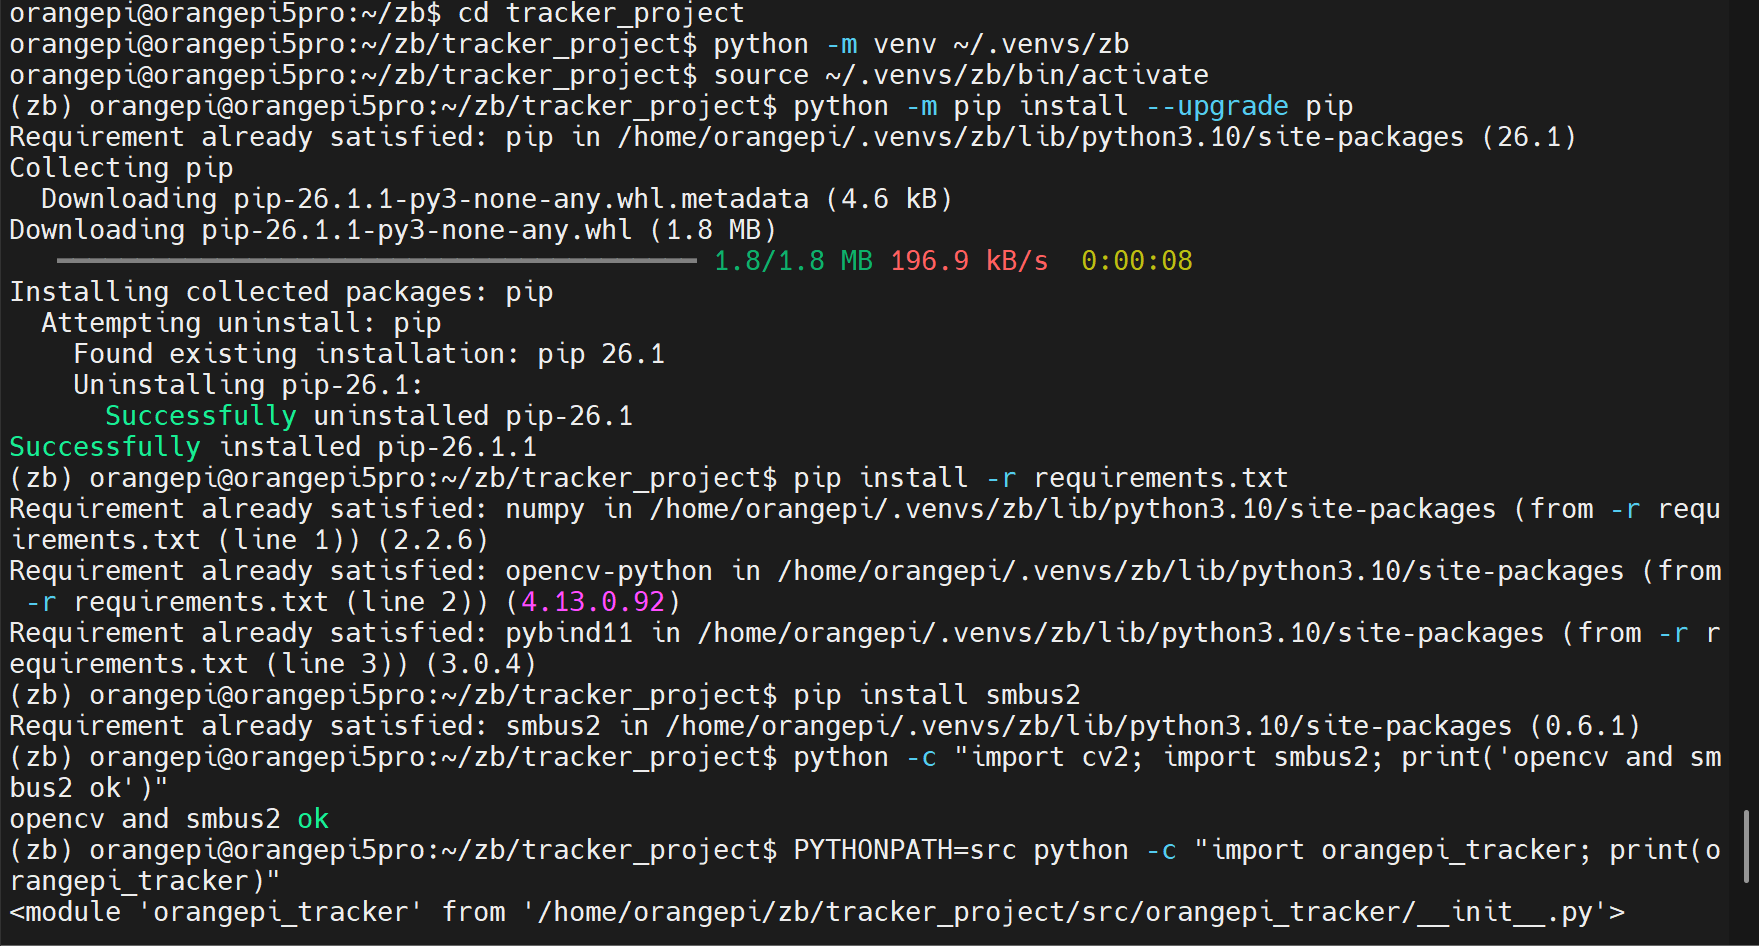
\includegraphics[width=0.86\linewidth]{figures/env_setup.png}
  \caption{OrangePi Python 环境配置}
  \label{fig:env-setup}
\end{figure}

\section{I2C 与 PCA9685 驱动}

由于系统中的 \texttt{i2cdetect} 工具曾出现 GLIBC 版本不匹配问题，项目实现了基于 smbus2 的 Python I2C 扫描脚本。调试结果表明，PCA9685 在 \texttt{/dev/i2c-1} 总线上可被识别，地址包括 \texttt{0x40} 和 \texttt{0x70}。I2C 扫描结果如图~\ref{fig:i2c-scan} 所示。

\begin{figure}[htbp]
  \centering
  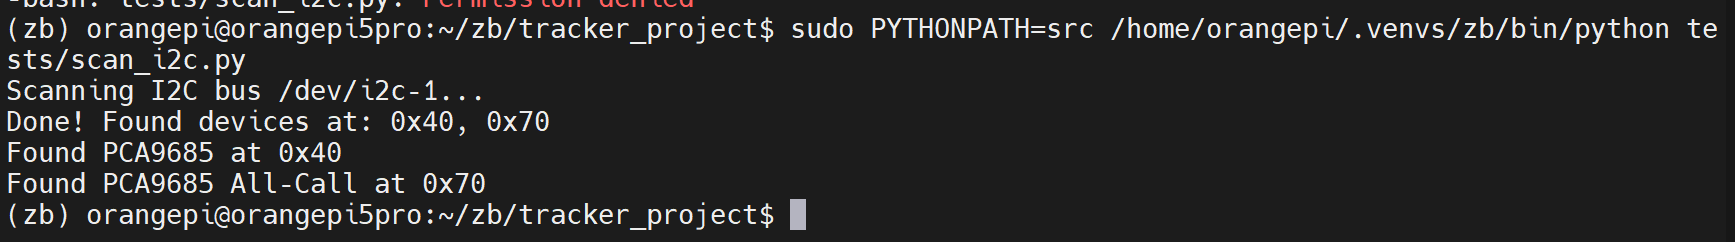
\includegraphics[width=0.86\linewidth]{figures/i2c_scan.png}
  \caption{I2C 扫描与 PCA9685 识别结果}
  \label{fig:i2c-scan}
\end{figure}

硬件驱动模块优先采用 \texttt{smbus2} 直接写 PCA9685 寄存器，完成 PWM 频率设置、脉宽映射和通道输出。若真实硬件不可用，程序可以回退到模拟硬件模式，便于在电脑端或无舵机条件下调试视觉流程。

\section{舵机测试}

舵机测试分为低层测试和主程序测试。低层测试直接调用 PCA9685 驱动通道输出固定角度，主程序测试则通过 \texttt{main.py --mode servo-test} 依次输出中心、水平最小、水平最大、俯仰最小、俯仰最大和回中动作。当前调试确认 channel 0 对应俯仰舵机，channel 1 对应水平舵机，主程序能够正常驱动云台运动。舵机测试终端输出如图~\ref{fig:servo-test} 所示。

\begin{figure}[htbp]
  \centering
  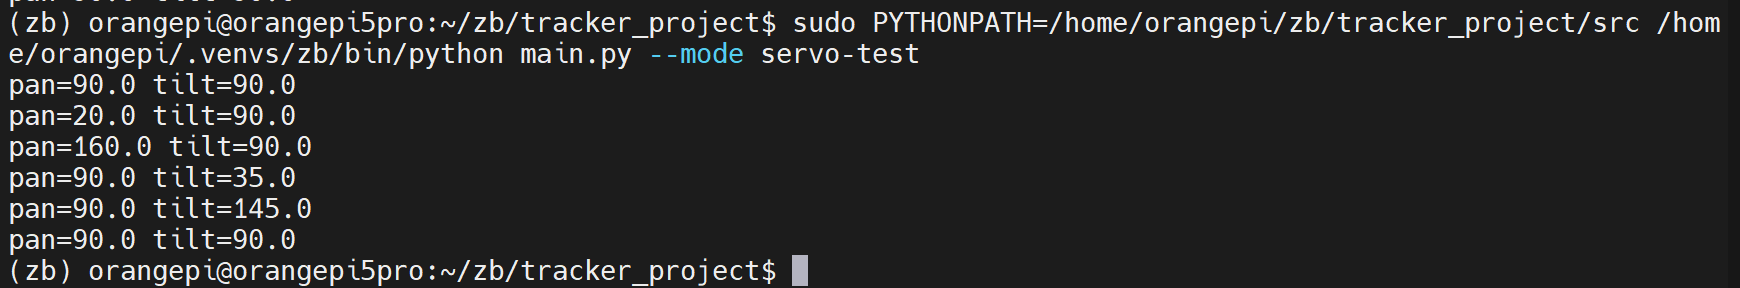
\includegraphics[width=0.86\linewidth]{figures/servo_test.png}
  \caption{舵机测试输出}
  \label{fig:servo-test}
\end{figure}

\section{视觉跟踪流程}

视觉检测模块首先对输入图像进行高斯模糊，然后转换到 HSV 色彩空间，根据红色目标阈值生成二值掩膜。随后对掩膜进行开闭运算去噪，并通过轮廓面积、面积比例和长宽比筛选候选目标。最终输出目标中心点、候选框、面积和置信度。

跟踪主程序在每一帧中执行检测、状态更新、控制输出和日志记录。为了方便调试，画面上叠加了目标框、中心点、画面中心线、状态、FPS 和云台角度等信息。跟踪测试终端输出如图~\ref{fig:tracking-terminal} 所示。

\begin{figure}[htbp]
  \centering
  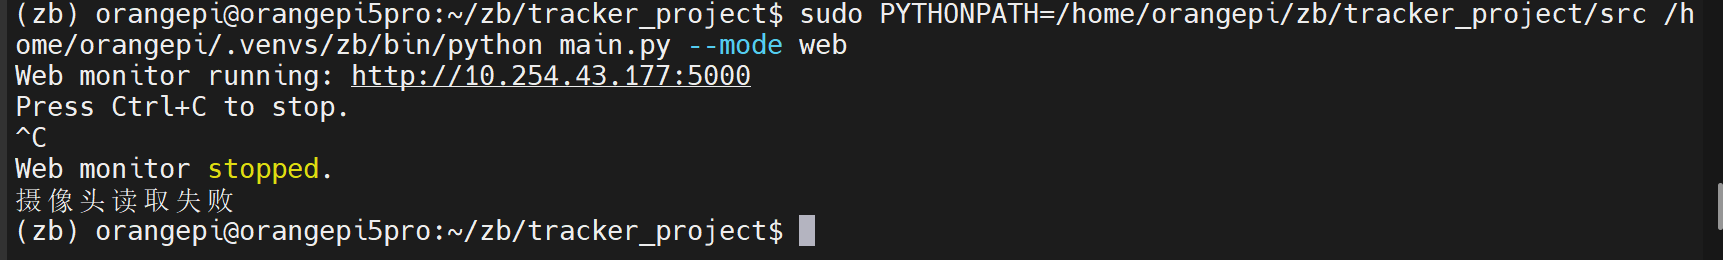
\includegraphics[width=0.86\linewidth]{figures/tracking_terminal.png}
  \caption{目标跟踪测试终端输出}
  \label{fig:tracking-terminal}
\end{figure}

\section{网页监控模式}

为解决 MobaXterm 远程调试时 OpenCV 图形窗口不稳定的问题，系统新增了网页监控模式。该模式使用 Python 标准库的 HTTP 服务提供页面，并通过 MJPEG 流输出实时图像。OrangePi 端启动 \texttt{main.py --mode web} 后，电脑浏览器访问终端打印的地址即可查看叠加后的实时画面。网页监控效果如图~\ref{fig:web-monitor} 所示。

\begin{figure}[htbp]
  \centering
  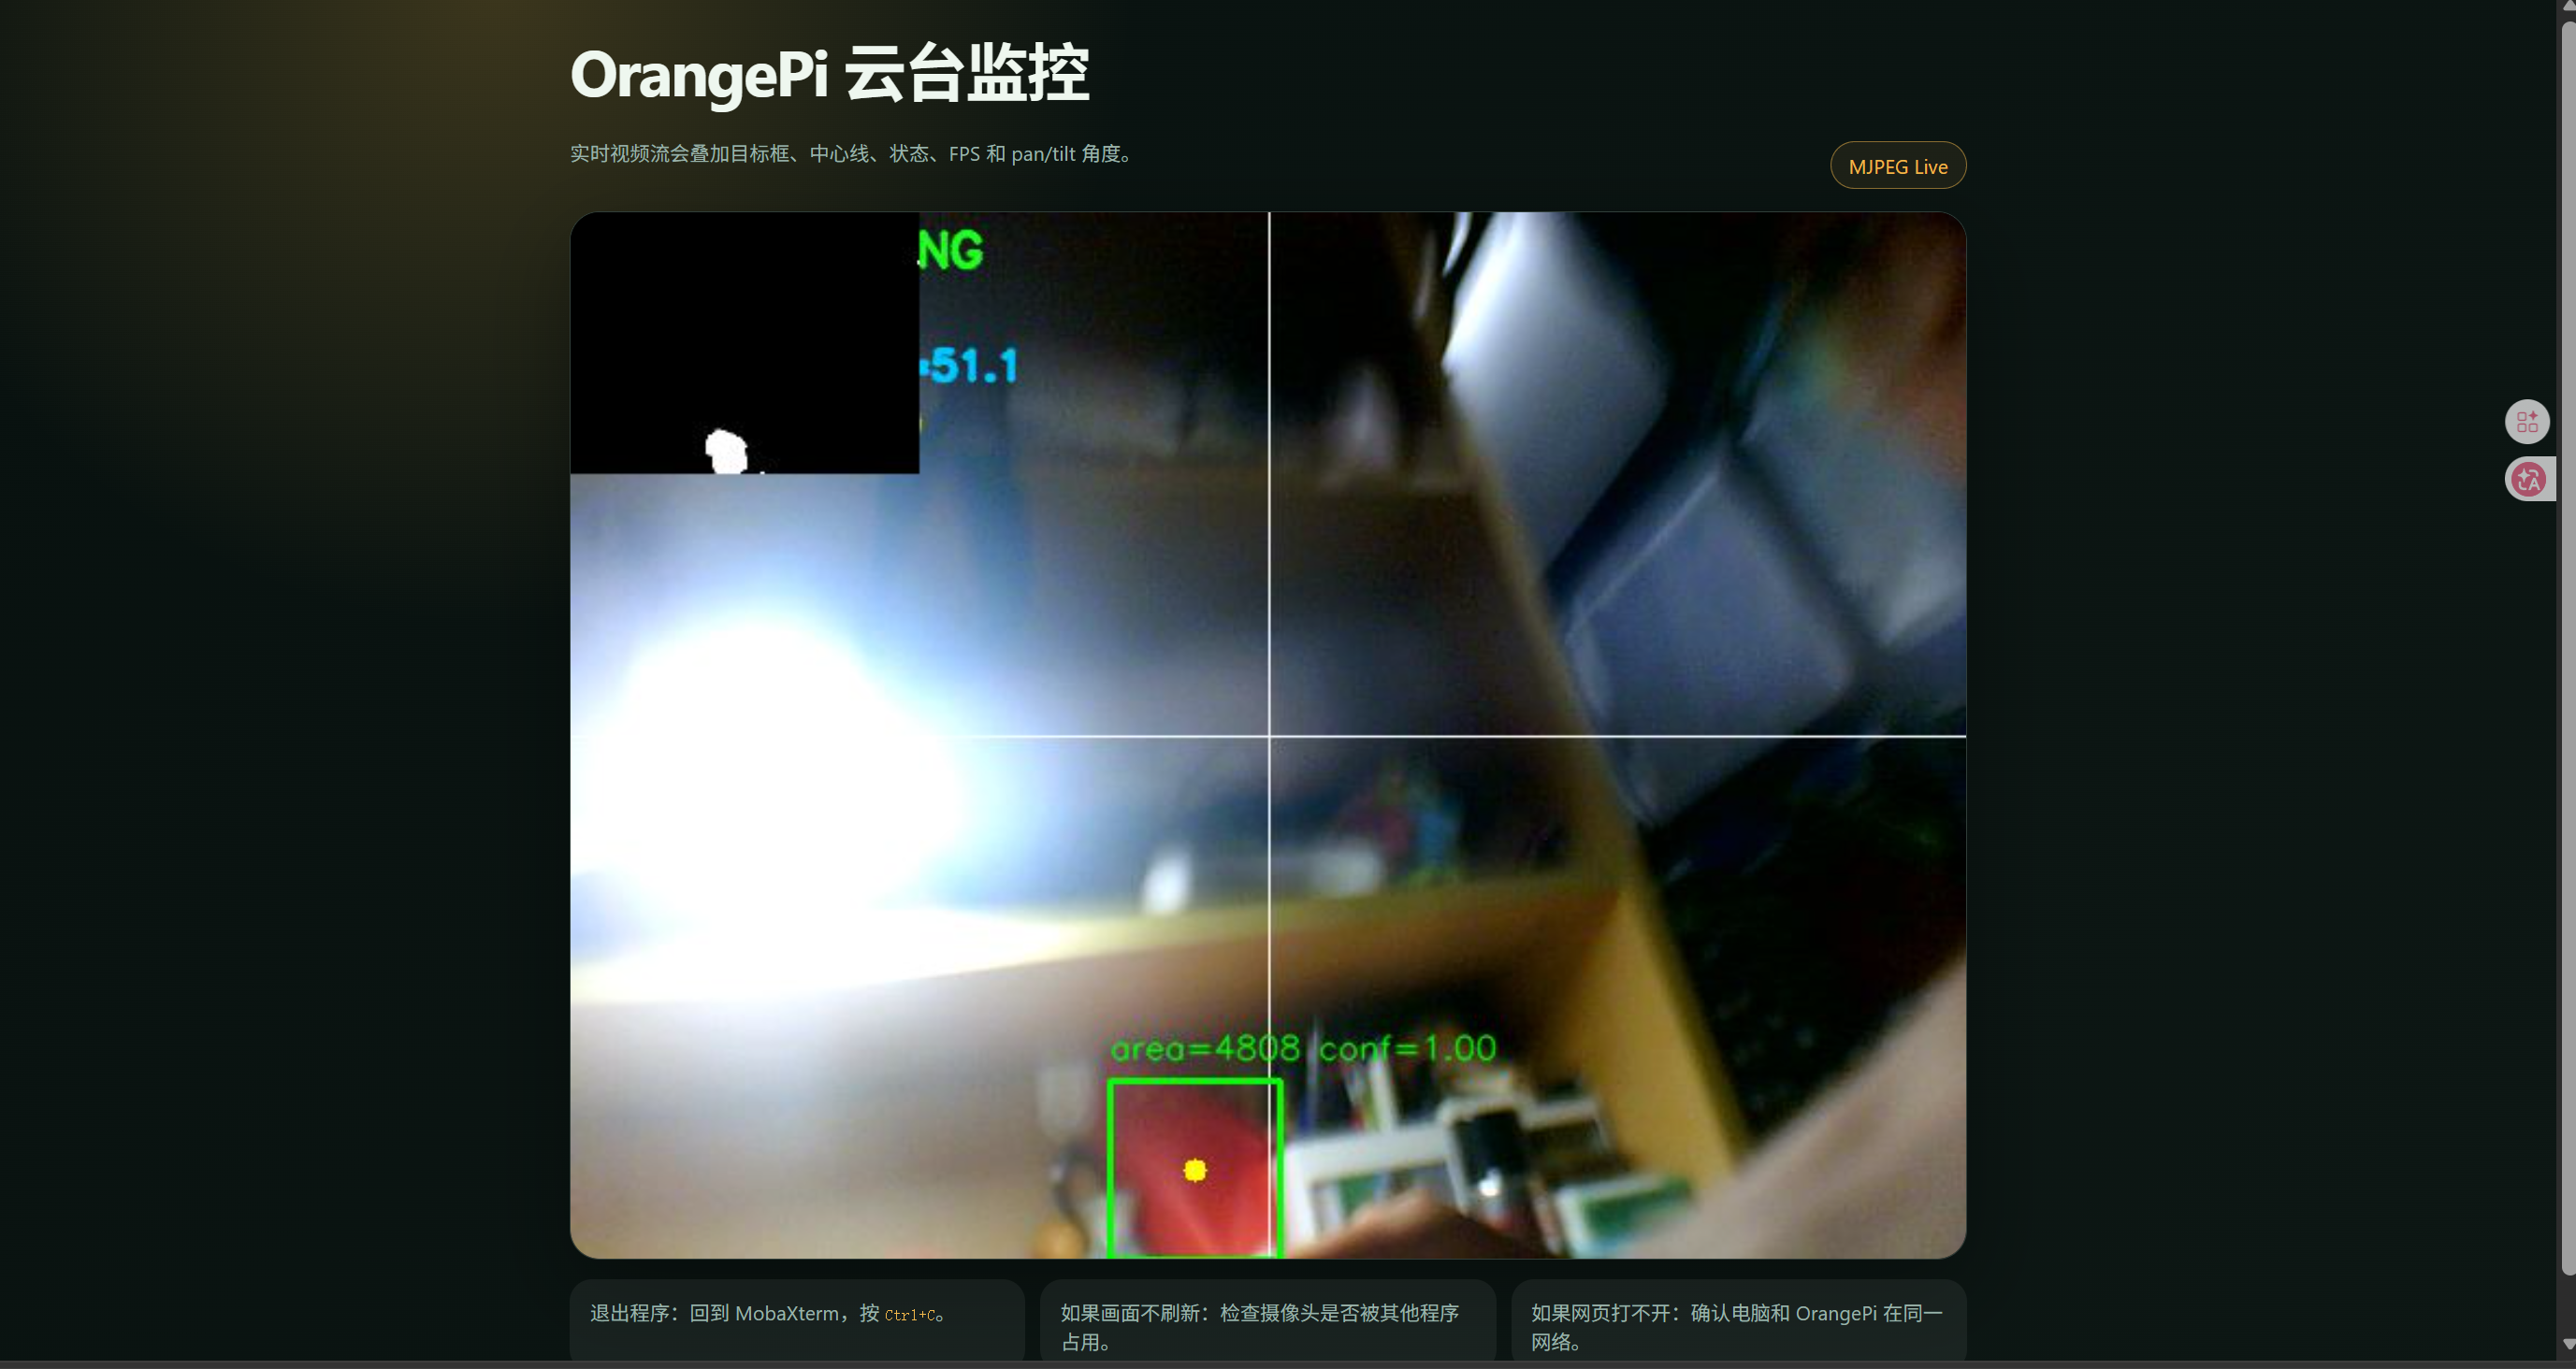
\includegraphics[width=0.92\linewidth]{figures/web_monitor.png}
  \caption{网页监控模式显示效果}
  \label{fig:web-monitor}
\end{figure}

为了降低调试风险，网页模式支持 \texttt{--simulate} 参数。使用模拟模式时程序只运行摄像头读取、目标检测和网页显示，不控制真实舵机，适合首次远程验证画面与识别效果。

